\documentclass{article}
\usepackage{amsmath}
\usepackage{mathtools}
\usepackage{gensymb}
\usepackage[a4paper,inner=1.5cm,outer=1.5cm,top=2cm,bottom=0.5cm]{geometry} 
\usepackage{xcolor}                    
\usepackage{tikz}                           
\usepackage{multicol}
\usepackage{pgfplots}
\usetikzlibrary{calc}
\usetikzlibrary{intersections}
\usetikzlibrary{intersections,calc,angles,quotes}
\usetikzlibrary{shapes,arrows,positioning,decorations.pathreplacing,calc}
\usetikzlibrary{calc,angles,positioning,intersections,quotes,decorations.markings}
\usepackage{tkz-euclide}
\usetikzlibrary{backgrounds}
\usetikzlibrary{calc,through}
\usetikzlibrary{angles}
\usetikzlibrary{fadings}
\usetikzlibrary{shapes.geometric}
\usetikzlibrary{shapes.symbols}
\usepackage{draftwatermark}
\usepackage{mathptmx}

\SetWatermarkText{\textcolor{black!10}{Mathema Shukur}}
\SetWatermarkFontSize{2 cm}
\usepackage[utf8]{inputenc}
\usepackage{fontspec}

\setmainfont{[Kalpurush.ttf]}
\newfontface{\en}{[Arial.ttf]} %%this is optional, if you want to use a secondary font. Any english font is supported
\newlength\Radius
\setlength\Radius{4cm}
\begin{document} 
	\Large
	\textcolor{red}{Welcome To} 
	\\
	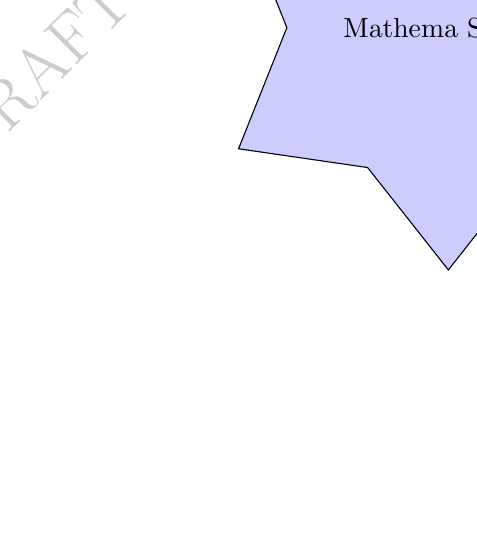
\begin{tikzpicture}
		\tikz \node [fill=blue!20,star,star points=6,draw] {Mathema Shukur };
	\end{tikzpicture}
	\\
	যাদের জন্যে প্রযোজ্যঃ  	\textcolor{magenta}{একাদশ ও দ্বাদশ শ্রেণীর শিক্ষার্থী} \\
	বিষয়ঃ \textcolor{magenta}{উচ্চতর গণিত ১ম পত্র} \\
	অধ্যায়ঃ \textcolor{magenta}{৩-সরলরেখা}\\ 
	Subtopicঃ  \textcolor{magenta}{  সমবিন্দু হওয়ার শর্ত কী ?  }\\
	\\
	যে বিন্দুতে দুইটি লাইন পরস্পরকে ছেদ করে তাকে ছেদ বিন্দু বলে (point of intersection)।  \\ 
	\\
	যে বিন্দুতে তিনটি লাইন পরস্পরকে ছেদ করে তাকে সমবিন্দু বলে (point of concurrency)। \\
	\\
	\textcolor{blue}{ তিনটি সরলরেখা সমবিন্দু হওয়ার শর্ত }(নির্ণায়কের মান শূন্য হবে)\\
	\begin{multicols}{2}
		\begin{align*}
			a_1x+b_1y+c_1&=0\\
			\\
			a_2x+b_2y+c_2&=0\\
			\\
			a_3x+b_3y+c_3&=0
		\end{align*}
		\\ 
		$	\begin{vmatrix}
			a_1 & b_1 &c_1\\
			\\
			a_2 & b_2 &c_2\\
			\\
			a_3 & b_3 &c_3
		\end{vmatrix}=0$\\ 
	\end{multicols}
	নির্ণায়কের ১ম কলামে $x$ এর সহগ \\
	\\
	নির্ণায়কের ২য় কলামে $y$ এর সহগ \\
	\\
	নির্ণায়কের ৩য় কলামে ধ্রুবক পদ \\
	\\
	\vspace{3cm}
	\\
	(BUET-2008-2009)\\
	$k$  এর মান কত হলে $x-y+5=0$,\quad $x+y-1=0$, এবং \quad $kx-y+13=0$ রেখাত্রয় সমবিন্দু হবে \\ 
	\begin{multicols}{2}
		\begin{align*}
			x-y+5&=0\\
			\\
			x+y-1&=0\\
			\\
			kx-y+13&=0
		\end{align*}
		\\ 
		\begin{align*}
			\begin{vmatrix}
				1& -1&5\\
				\\
				1 & 1 &-1\\
				\\
				k& -1 &13
			\end{vmatrix}&=0\\
			\\
			(1)	\begin{vmatrix}
				1 &-1\\
				\\
				-1 &13
			\end{vmatrix}-(-1)	\begin{vmatrix}
				1 &-1\\
				\\
				k &13
			\end{vmatrix}+(5)	\begin{vmatrix}
				1 &1\\
				\\
				k &-1
			\end{vmatrix}&=0\\
			\\
			1(13-1)+1(13+k)+5(-1-k)&=0\\
			\\
			12+13+k-5-5k&=0\\
			\\
			-4k+20&=0\\
			\\
			k&=5
		\end{align*}
	\end{multicols}
	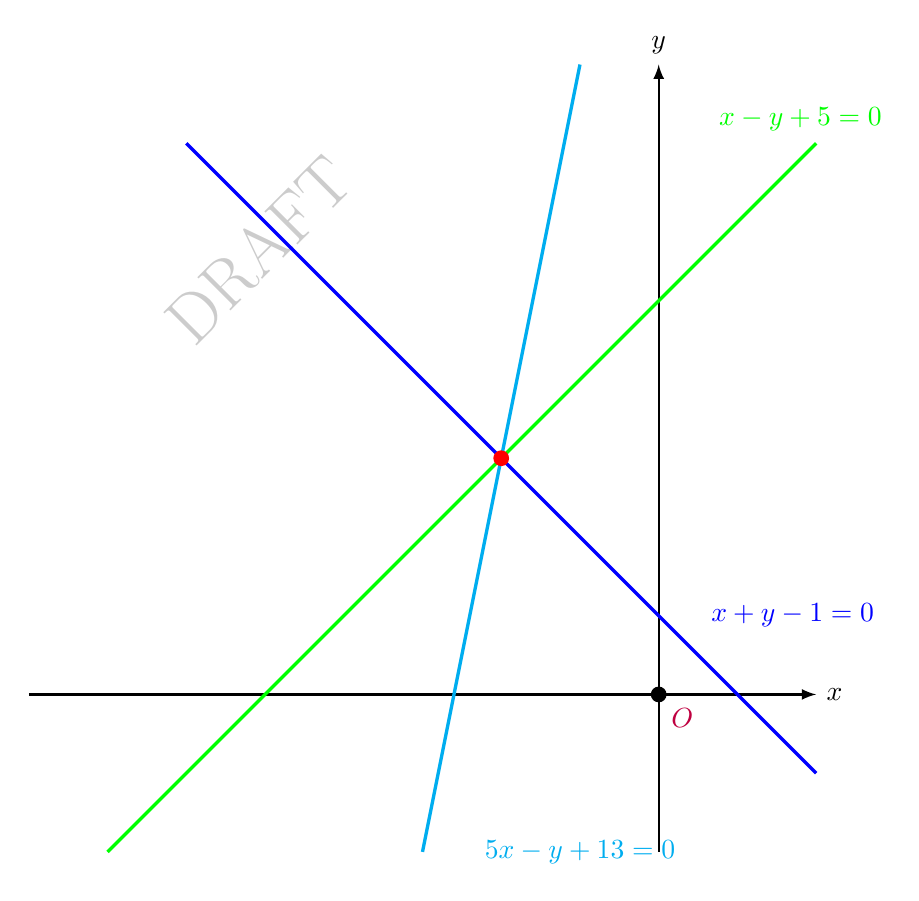
\begin{tikzpicture}[transform shape,scale=1]
		\draw [-latex,thick](-8,0) -- (2,0) node[right] {$x$} coordinate(x axis);
		\draw [-latex,thick](0,-2) -- (0,8) node[above] {$y$} coordinate(y axis);
		\fill[black] (0,0) circle (1 mm);
		\node at (0.3,-0.3) {$\textcolor{purple}{O}$};	
		\node at (1.7,1) {$\textcolor{blue}{x+y-1=0}$};	
		\node at (1.8,7.3) {$\textcolor{green}{x-y+5=0}$};
		\node at (-1,-2) {$\textcolor{cyan}{5x-y+13=0}$};		
		\draw[very thick,green] (2,7)--(-7,-2);	
		\draw[very thick,blue] (2,-1)--(-6,7);	
		\draw[very thick,cyan] (-1,8)--(-3,-2);	
		\fill[red] (-2,3) circle (1 mm);
	\end{tikzpicture}
	\\
	ঢাকা বিশ্ববিদ্যালয় ভর্তি পরীক্ষা- ২০১৪-২০১৫\\ 
	তিনটি সরলরেখা $3x+5y=2$,\quad $2x+3y=0$,\quad $ax+by+1=0$ সাধারণ বিন্দুগামী হলে  $a$ এবং  $b$ এর মধ্যে সম্পর্ক নির্ণয় কর \\ 
	\begin{multicols}{2}
		\begin{align*}
			3x+5y-2&=0\\
			\\
			2x+3y&=0\\
			\\
			ax+by+1&=0
		\end{align*}
		\\ 
		\begin{align*}
			\begin{vmatrix}
				3& 5&-2\\
				\\
				2 & 3 &0\\
				\\
				a& b &1
			\end{vmatrix}&=0\\
			\\
			(3)	\begin{vmatrix}
				3 &0\\
				\\
				b &1
			\end{vmatrix}-(5)	\begin{vmatrix}
				2 &0\\
				\\
				a &1
			\end{vmatrix}+(-2)	\begin{vmatrix}
				2 &3\\
				\\
				a &b
			\end{vmatrix}&=0\\
			\\
			3(3-0)-5(2-0)-2(2b-3a)&=0\\
			\\
			9-10-4b+6a&=0\\
			\\
			6a-4b-1&=0\\
			\\
			6a-4b&=1
		\end{align*}
	\end{multicols}
	ঢাকা বোর্ড-২০১৪\\ 
	$ax+by+c=0$,\quad$bx+cy+a=0$,\quad $cx+ay+b=0$ রেখাত্রয় সমবিন্দু হলে দেখাও যে,  $a+b+c=0$\\ 
	\\
	\begin{align*}
		ax+by+c&=0\\
		\\
		bx+cy+a&=0\\
		\\
		cx+ay+b&=0
	\end{align*}
	\\ 
	\begin{align*}
		\begin{vmatrix}
			a& b&c\\
			\\
			b & c &a\\
			\\
			c& a &b
		\end{vmatrix}&=0\\
		\\
		(a)	\begin{vmatrix}
			c &a\\
			\\
			a &b
		\end{vmatrix}-(b)	\begin{vmatrix}
			b &a\\
			\\
			c &b
		\end{vmatrix}+(c)	\begin{vmatrix}
			b &c\\
			\\
			c &a
		\end{vmatrix}&=0\\
		\\
		a(bc-a^2)-b(b^2-ac)+c(ab-c^2)&=0\\
		\\
		abc-a^3-b^3+abc+abc-c^3\\
		\\
		a^3+b^3+c^3-3abc&=0\\
		\\
		\frac{1}{2}(a+b+c)\{(a-b)^2+(b-c)^2+(c-a)^2\}&=0\\
		\\
		(a+b+c)=0,\quad \{(a-b)^2+(b-c)^2+(c-a)^2\}&\ne 0
	\end{align*}
\end{document}